\section{Introduction}

\begin{frame}
\frametitle{Introductions}

\begin{itemize}
\item Daniel Blezek, Ph.D., Mayo Clinic
\item Luis Ib\'a\~nez, Ph.D., Kitware
\item Hans Johnson, Ph.D., University of Iowa
\item Bradley Lowekamp, Lockheed Martin (National Library of Medicine)
\end{itemize}

\end{frame}

\begin{frame}
\frametitle{Tutorial Goals}
\begin{itemize}
\item Gentle introduction to ITK
\item Introduce SimpleITK
\item Provide hands-on experience
\item Problem solving, not direction following
\item ...but please follow directions!
\end{itemize}
\end{frame}

\begin{frame}
\frametitle{ITK Overview}
How many are familiar with ITK?
\end{frame}

\begin{frame}
\frametitle{Ever seen code like this?}
\begin{center}
\lstcpp
\lstinputlisting{Code/DiscreteGaussianFilter.cxx}
\end{center}
\end{frame}

\begin{frame}
\frametitle{What if you could write this?}
\begin{center}
\lstpython
\lstinputlisting{Code/DiscreteGaussianFilter.py}
\end{center}
\pause
We are here to tell you that you can...
\end{frame}

\begin{frame}{Goals of SimpleITK}
\begin{itemize}
\item Be an ``on-ramp'' for ITK
\item Simplify the use of ITK by
  \begin{itemize}
  \item Providing a templateless, typeless layer for ITK in C++
  \item Providing wrappings in scripting languages
  \item Providing access to most ITK algorithms
\end{itemize}
\end{itemize}
\end{frame}

\begin{frame}{SimpleITK Architectural Overview}
\begin{itemize}
\item Conceptually, SimpleITK is an application library built on ITK
\item All functionality provided by ITK
\item Components:
  \begin{itemize}
    \item Template expansion system
    \item C++ library
    \item Small SWIG definition (more details later)
    \item ``Glue'' code for several scripting languages
    \item Some language utilities
  \end{itemize}
\item Open Source, Apache licensed project (\url{http://www.opensource.org/licenses/apache2.0.php})
\item Hosted by GitHub (\url{https://github.com/SimpleITK/SimpleITK})
\end{itemize}
\end{frame}

\begin{frame}{Templates in ITK}
\begin{center}
\lstcpp
\lstinputlisting{Code/ITKTemplateSample.cxx}
\end{center}
\end{frame}

\begin{frame}
\frametitle{Template Freedom}
\begin{center}
\lstcpp
\lstinputlisting{Code/SimpleITKTemplatelessSample.cxx}
\end{center}
\end{frame}

\begin{frame}
\frametitle{Programming Models}
\begin{itemize}
\item Object oriented
\item Function oriented
\end{itemize}
More about this later
\end{frame}

\begin{frame}
\frametitle{Wrapping}
Transformed by SWIG
\begin{itemize}
\item Parses header and ``interface'' files
\item Automatically creates scripting ``glue''
\item Wrappings available for:
\begin{itemize}
  \item Python
  \item Java
  \item C\#
  \item Tcl, Lua, Ruby
  \item Others as requested\dots
\end{itemize}
\end{itemize}
\end{frame}


\begin{frame}{Image Anatomy}
\begin{center}
  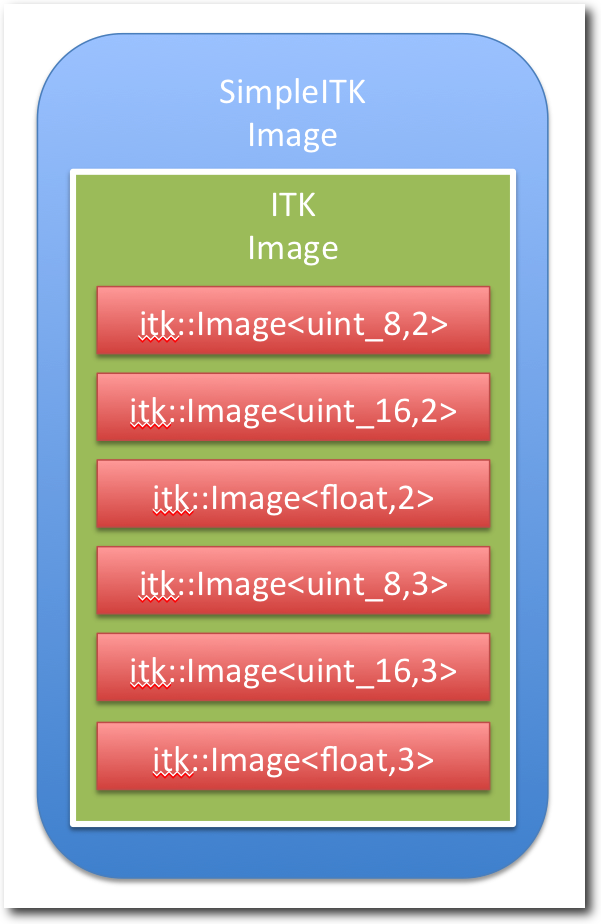
\includegraphics[width=0.3\textwidth]{Images/SimpleITKImageAnatomy_shadow}
\end{center}
\begin{itemize}
  \item SimpleITK images contain \texttt{itk::Image}
  \item Hides the templates
  \item Adds useful ``utility'' functions
\end{itemize}
\end{frame}

\begin{frame}{Filter Anatomy}
\begin{center}
  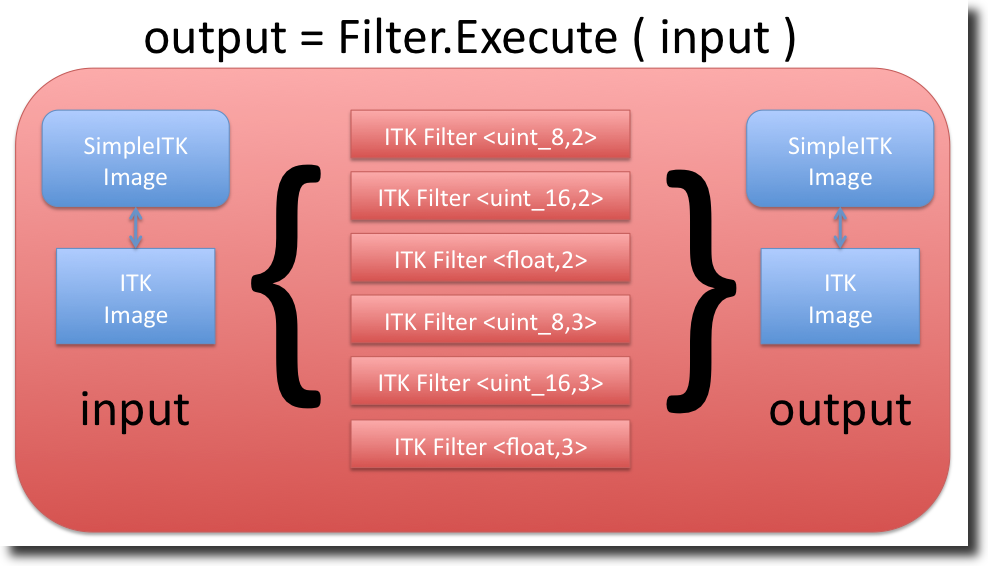
\includegraphics[width=0.7\textwidth]{Images/FilterInternals_shadow}
\end{center}
\begin{itemize}
  \item SimpleITK filters contain \texttt{itk::ImageToImageFilter}
  \item Hides the templates
  \item Adds useful ``utility'' functions
  \item (Mainly) \texttt{output = Filter.Execute ( input )}
\end{itemize}
\end{frame}



% LocalWords:  SimpleITK typeless ITK
